\chapter{绪论}

\section{研究背景与意义}
近年来,随着各种社交媒体和论坛的发展,互联网上的影评已经成为了观影者表达观点、进行交流的重要方式。互联网上出现了许多以影评为主要内容的网站、社区,如IMDB,Rotten Tomatoes,以及中文的豆瓣等。在这些网站上每天都产生出大量的来自用户的文本。这些文本中往往包含了丰富的用户情感信息,如用户对某个电影、演员的评价等。这些用户生成的文本是网站了解用户观点,电影制作者进行市场调研的重要资源。

豆瓣、IMDB上的影评都带有对应的评分(打星数),这样的“影评—评分”对可以看做有标注的数据,它们不需要进一步的人工标注,就可以被用作情感分析的语料。另一些博客或论坛性质的网站,则没有要求用户在给出评论的同时打分。图1.1为一些来自互联网的影评示例。
\begin{figure}[ht]
\centering

\includegraphics[width=10cm]{Reviews}
\caption{上、中:带有对应评分的影评,分别来自豆瓣和IMDB;下:没有评分的影评,来自知乎} \label{fig:Reviews}
\end{figure}

对影评进行情感分析,将文本形式的影评转化为对应的评分预测,对于网站了解用户对于电影的评价、获得用户反馈和针对用户进行推荐都有着重要意义。在网站不要求用户在评论的同时给出评分的情景下,文本是获得用户情感信息的唯一途径。分析用户文本远不如分析量化的评分容易,如果要人工进行统计分析,工作量会非常大。因此,使用算法对影评进行情感分析,从用户文本中预测该用户对电影的评分,可以大大帮助网站分析来自于用户的数据,收集用户对某一部电影的量化评价。量化后的影评数据方便进行统计,也可以帮助电影制作者进行市场调查。此外,一个用户对各个电影的评分的预测可以很好 地体现该用户的特征,评分预测的结果可以用作推荐系统的输入数据,使网站针对每个用户投放的推荐更为准确。

对于既有影评,又要求用户同时对电影打分的网站,对影评进行情感分析仍然有很重要的意义。因为每个用户对于分数的理解有很大差别,有些用户认为三星是“不错”、“满意”的评分,而另一些则认为是“不满意”、“相当差”。故单纯基于用户打分来收集的对电影的评价往往是有一些偏差的。对文本影评进行情感分析的结果可以在原有评分的基础上起到一个平滑(smooth)的作用,使统计数据更加准确。



\section{相关研究现状}
文本情感分析一直是自然语言处理方向研究的热点,现代进行文本情感分析的方法一般有基于词库(或基于知识)的方法、基于机器学习的有监督学习和无监督学习的方法、以及基于深度学习的方法。

基于词库的文本情感分析方法会采用已知的情感词典(一般由人工筛选出常见的带有情感色彩的单词并进行标注),对于每一个句子,根据其包含的情感单词以及句子的语法结构计算该句的情感倾向\cite{taboada.2011.lexicon}。

现有的机器学习的方法被广泛应用于文本情感分析的问题。监督学习的方法如朴素贝叶斯、最大熵和支撑向量机等,都可以用于情感分析。Pang 等人使用这些方法在来自IMDB的英文影评数据上进行了二分类的实验,其结果证明使用单个单词(unigram)作为特征进行分类就可以取得很好效果,支撑向量机在3折交叉验证中取得了82.9\%的准确率\cite{Pang.2002.ml}。

非监督学习的方法也被应用于情感分析,Peter D. Turney等人使用一种基于情感极性(Sentiment Orientation)的非监督的方法\cite{turney.2002.thumbs}。一个句子的分类由它包含的所有短语的情感方向的平均值决定。每个短语的情感方向由它与单词excellent和poor的相互信息(mutual information)决定。该方法在来自Epinions的410条评论上进行了验证,取得了74\%的准确率。

深度学习的模型也被越来越多地应用于情感分析。卷积神经网络(Convolutional Neural Network, 简称CNN)是一种最早发源于计算机图形学的深度学习模型。Yoon Kim等人使用将单词转化为词向量,再用词向量组成的矩阵来模拟图形矩阵的方法,将卷积神经网络应用在了文本分类的问题上\cite{kim.2014.convolutional}。Yoon等人使用一个简单的只有一层卷积层的卷积神经网络在6个数据集上进行了实验,均取得了很好的效果。

\section{本论文主要内容}
本论文使用来自豆瓣的中文短评(每条长度不超过140字,带有评分,可以看作有标注的数据)作为语料,使用卷积神经网络等方法进行文本情感分析,由影评预测对应的评分。

\begin{figure}[ht]
\centering
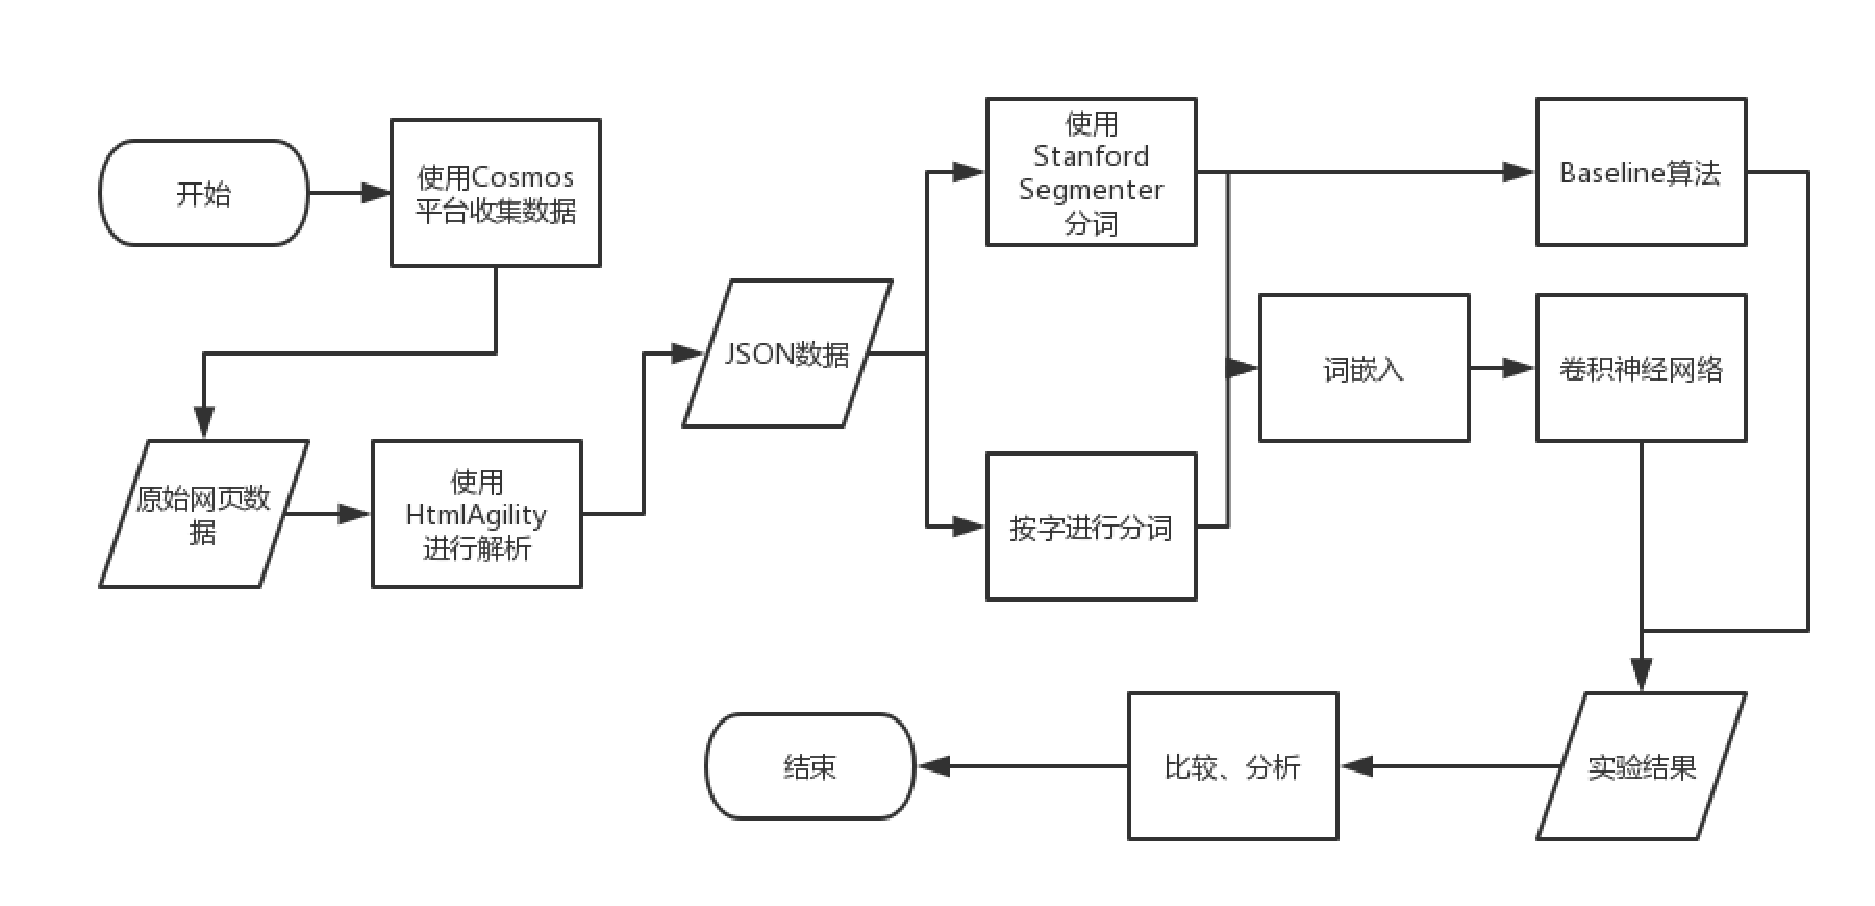
\includegraphics[width=15cm]{Flowchart}
\caption{本论文实验流程图} \label{fig:Flowchart}
\end{figure}


1.	收集数据。使用微软必应搜索的Cosmos分布式处理平台获取了来自豆瓣的16万短评数据以及10万长评数据。

2.	数据预处理。进行中文分词,使用Word2vec算法训练出中文单词的词嵌入

3.	建立深度学习模型,调整网络结构,找到适合中文影评数据的模型;实现朴素贝叶斯等传统算法,作为比较。

4.	比较和分析实验结果

本文的组织如下:第一章为绪论,介绍选题的背景和意义,简述当前相关领域研究状况和本论文主要工作;第二章介绍了文本情感分析的相关定义,以及基于词库的方法和基于机器学习的方法;第三章介绍了深度学习的方法在文本情感分析问题上的应用,详细介绍了用于文本分类的卷积神经网络,包括其模型细节和具体算法;第四章介绍了使用卷积神经网络进行影评分类实验的数据集和实验设置,列出了实验结果,对baseline实验以及多组卷积神经网络的实验结果进行了对比和分析;第五章进行了全文总结和未来工作的展望。
